\documentclass[ecta]{econsocart}
\usepackage{amsmath,amssymb,booktabs,natbib,pdfpages,hyperref}
\hypersetup{hidelinks,hypertexnames=false,pdftitle={Neural Bellman Operators -- R10 Preservation Supplement},pdfauthor={Qian QI}}
\begin{document}
\begin{frontmatter}
\title{Neural Bellman Operators: Preservation Supplement to Revision R10}
\runtitle{NBO: R10 Preservation Supplement}
\begin{aug}
\author[id=au1,addressref={add1}]{\fnms{Qian}~\snm{QI}\ead[label=e1]{qiqian@pku.edu.cn}}
\address[id=add1]{\orgname{Peking University}}
\end{aug}
\begin{abstract}
The current paper and proofs are in ECTA\_R10. This supplement preserves the complete completed R9 paper and the entire R9 preservation supplement without deleting equations, numerical tables, counterexamples, or unsuccessful calculations. Earlier precision statements are dated results, not current R10 claims. All underlying historical sources remain unchanged in the revision branch.
\end{abstract}
\end{frontmatter}
\section*{Reading map}
The R10 paper contains the affine-preference dual, its complete verification proof, the original-model certificates below .01, the quantitative output-error allowance, the economic cost comparisons, and every main R9 theorem or its explicitly preserved appendix counterpart. A separate point-by-point response to the R9 referee accompanies the paper in the R10 revision directory.

The following pages reproduce the completed R9 paper, including its older .10634 flexible-policy bound. They are followed by the complete R9 supplement, which preserves R8, R4, the delivered R5 numerical material, recursive utility, sophisticated temporal selves, games, stochastic-trace identities, finite safeguards, and historical diagnostics. Historical claims must be read with their original version labels. The R10 current status is determined by its own theorem, result files, and source/result/build manifest, not by the older precision flags reproduced here.

\section*{Part I: Completed R9 paper, preserved in full}
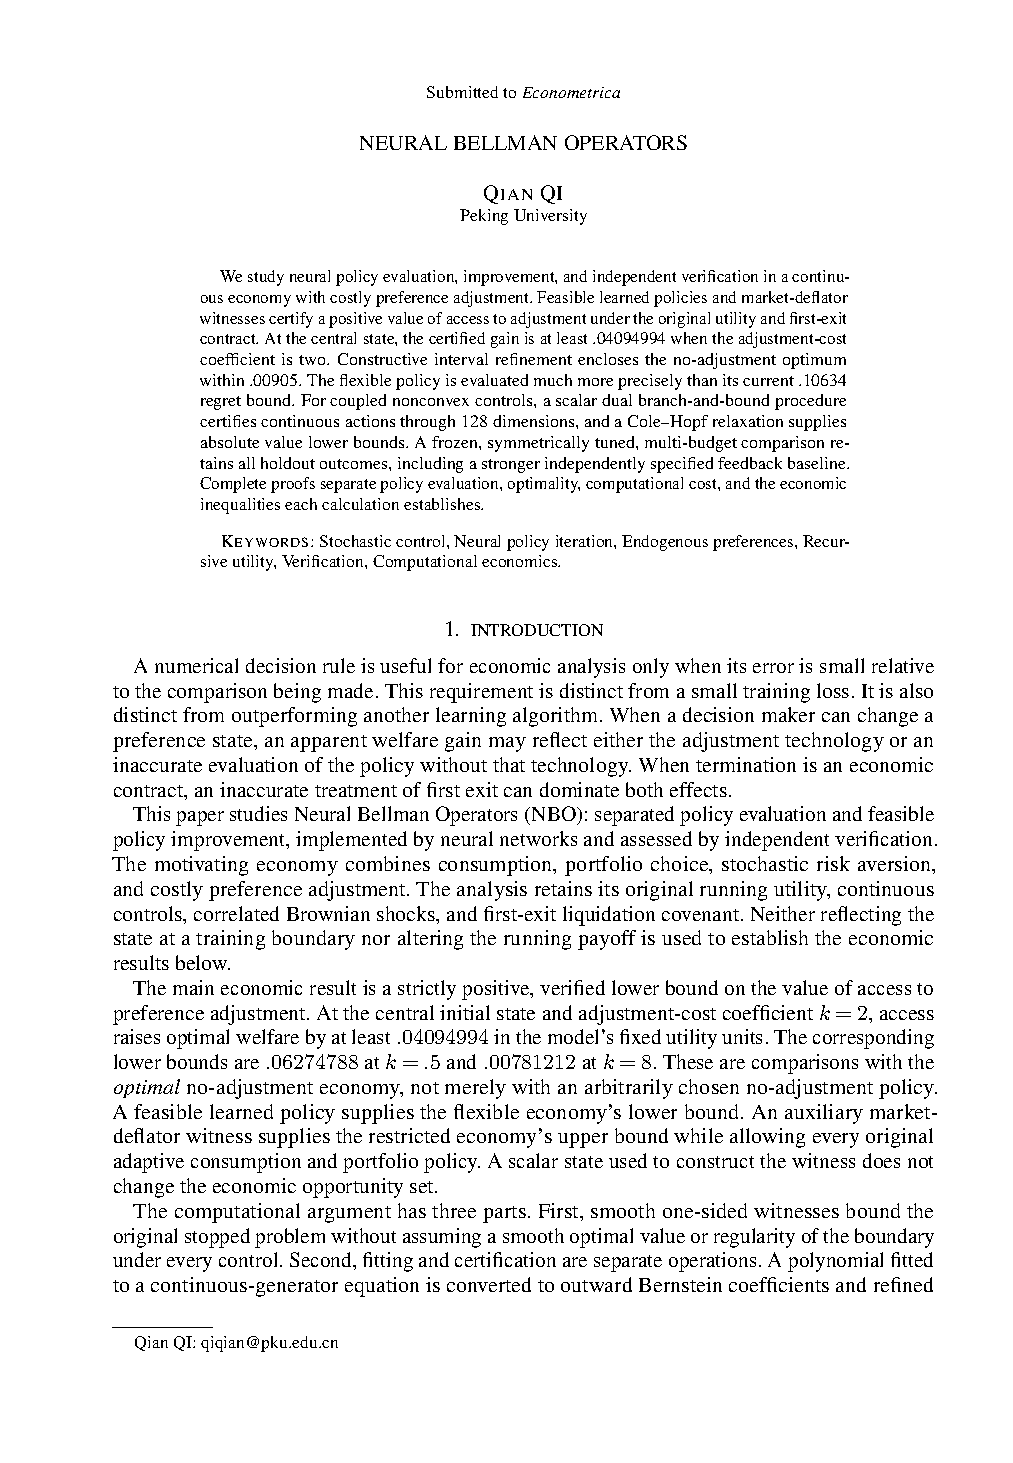
\includepdf[pages=-,pagecommand={},fitpaper=true]{ECTA_R9.pdf}
\section*{Part II: Completed R9 supplement, preserved in full}
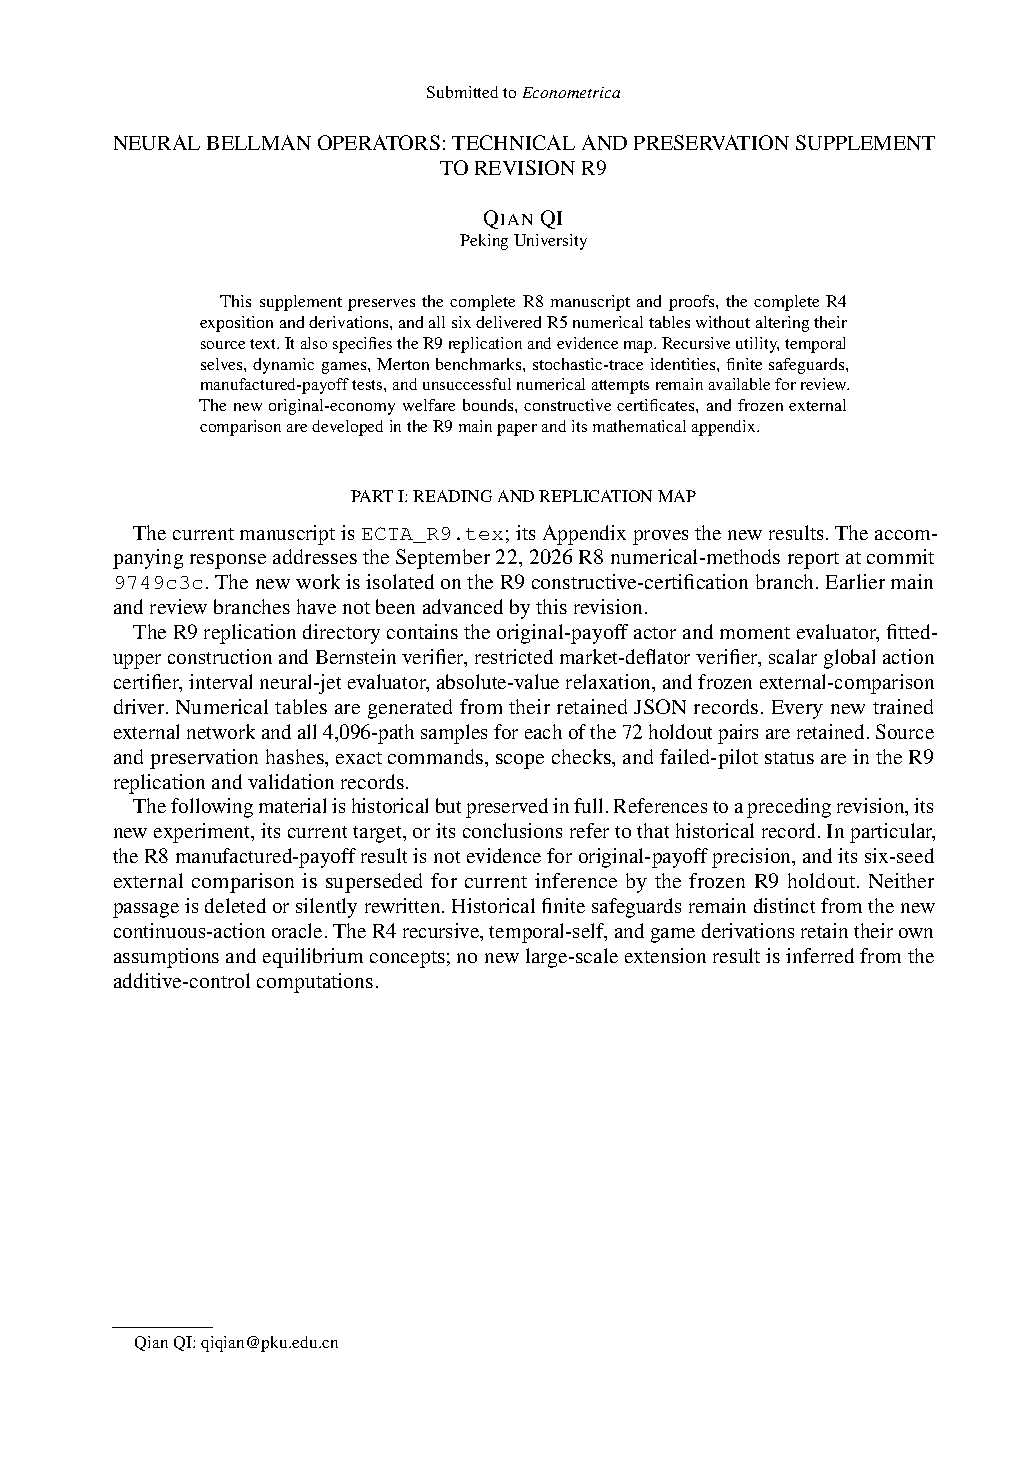
\includepdf[pages=-,pagecommand={},fitpaper=true]{SUPP_R9.pdf}
\end{document}
